% ============================================================
% CHAPTER 4 -- SYSTEM DESIGN
% FEMCARE: An AI-Powered Women's Reproductive Health Platform
% ============================================================

\chapter{System Design}\doublespacing
\label{chap:design}

% ------------------------------------------------------------
\section{Introduction}
\label{sec:design-intro}

This chapter describes the design of the FEMCARE system: how its components are structured, how they interact, how data is organised in the database, and how the key workflows are realised. The requirements established in Chapter 3 are the basis for the design decisions described here. Implementation details, source-code-level logic, and testing are addressed in subsequent chapters.

% ------------------------------------------------------------
\section{System Architecture}
\label{sec:architecture}

FEMCARE follows a three-tier client--server architecture comprising a presentation tier, a logic tier, and a data tier, supplemented by three external cloud services.

\begin{itemize}
    \item \textbf{Presentation Tier} -- A React single-page application (SPA) built with Vite. The frontend handles all user interaction, client-side routing via React Router DOM, and communicates with the backend and database through HTTP and the Supabase JavaScript client.

    \item \textbf{Logic Tier} -- A Python FastAPI backend served by Uvicorn. This tier handles ML inference, AI chatbot requests, appointment booking operations, and administrative tasks such as email auto-confirmation. It is the only tier that holds service-role credentials and API keys.

    \item \textbf{Data Tier} -- A Supabase-managed PostgreSQL database that stores all user health data. Supabase Authentication manages user identity and JWT issuance. Row Level Security (RLS) policies enforce per-user data isolation at the database level.

    \item \textbf{External Services} -- Three cloud services are integrated: the Groq API provides LLM inference for the AI health assistant; the Resend API delivers transactional appointment emails; and OpenStreetMap tiles (rendered via Leaflet) provide the interactive provider map.
\end{itemize}

The communication paths between tiers are shown in Table~\ref{tab:arch-comms}. Figure~\ref{fig:architecture} shows the overall system architecture of FEMCARE.

\begin{figure}[h!]
\centering
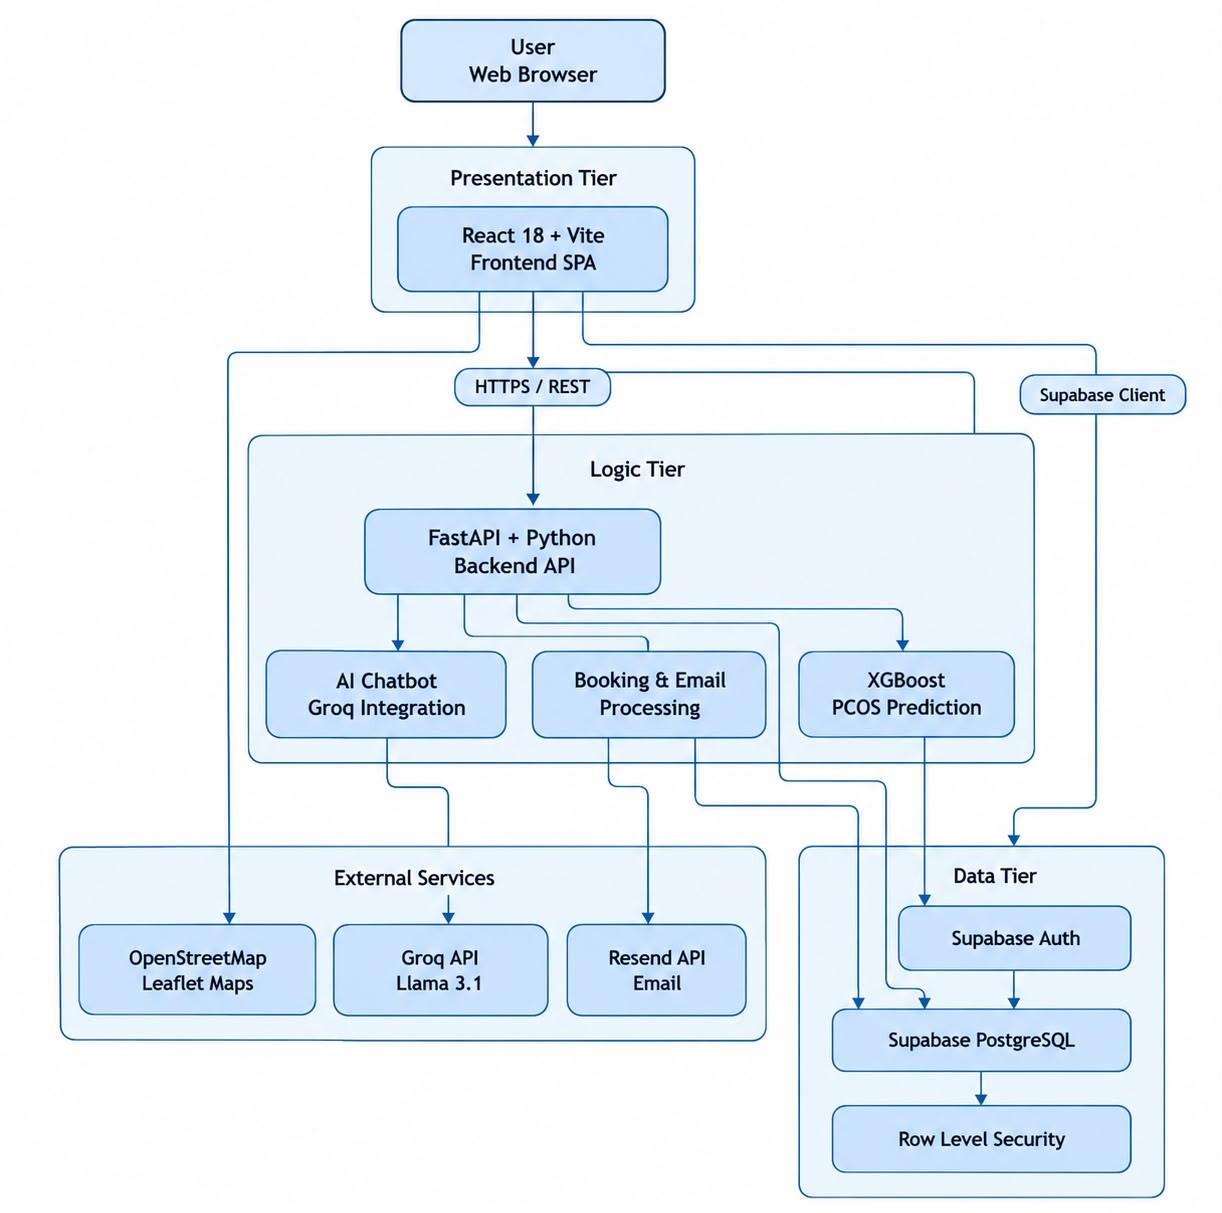
\includegraphics[width=0.90\textwidth]{4.1.jpeg}
\caption{System Architecture of FEMCARE}
\label{fig:architecture}
\end{figure}

\begin{table}[h!]
\centering
\caption{Inter-Tier Communication}
\label{tab:arch-comms}
\renewcommand{\arraystretch}{1.4}
\begin{tabular}{|p{3.2cm}|p{3.2cm}|p{3cm}|p{3cm}|}
\hline
\rowcolor[HTML]{D9D9D9}
\textbf{From} & \textbf{To} & \textbf{Protocol} & \textbf{Credential} \\
\hline
React Frontend & Supabase DB & HTTPS (supabase-js) & Anon key + JWT \\
\hline
React Frontend & FastAPI Backend & HTTPS REST (fetch) & Bearer JWT (optional) \\
\hline
FastAPI Backend & Supabase DB & HTTPS (supabase-py) & Service role key \\
\hline
FastAPI Backend & Groq API & HTTPS & GROQ\_API\_KEY \\
\hline
FastAPI Backend & Resend API & HTTPS (httpx) & RESEND\_API\_KEY \\
\hline
\end{tabular}
\end{table}

A key architectural decision is the dual access path to Supabase. The frontend queries Supabase directly for cycle data, period records, and symptom history using the anon key; RLS policies automatically restrict these queries to the authenticated user's own rows. The backend uses the service role key, which bypasses RLS, only for operations that require elevated access -- specifically booking management and email confirmation -- where server-side identity verification has already been performed.

% ------------------------------------------------------------
\section{Module Design}
\label{sec:modules}

FEMCARE is organised into eight functional modules. Table~\ref{tab:modules} summarises each module and its primary responsibility.

\begin{table}[h!]
\centering
\caption{FEMCARE Module Summary}
\label{tab:modules}
\renewcommand{\arraystretch}{1.4}
\begin{tabular}{|p{3.8cm}|p{3.5cm}|p{5.5cm}|}
\hline
\rowcolor[HTML]{D9D9D9}
\textbf{Module} & \textbf{Primary Files} & \textbf{Responsibility} \\
\hline
Authentication & AuthContext.jsx & Registration, login, session management, profile loading \\
\hline
Cycle Tracking & LogCycle.jsx, cycleService.js, symptomService.js & Daily logging of flow, pain, mood, and symptoms \\
\hline
Dashboard & Dashboard.jsx & Real-time cycle phase, health summary, compact chatbot \\
\hline
PCOS Assessment & HealthAssessment.jsx, main.py (/api/predict) & 18-feature quiz, ML prediction, result display \\
\hline
AI Health Assistant & ChatBot.jsx, femcare\_chatbot.py & Scoped LLM chatbot with user-context enrichment \\
\hline
Find Care \& Booking & FindCare.jsx, main.py (/api/book-appointment) & Provider map, slot selection, booking, cancellation \\
\hline
Health Awareness & Awareness.jsx, awarenessData.js & Condition content, warning signs, prevention habits \\
\hline
Email Notification & femcare\_email.py & Confirmation and cancellation emails via Resend API \\
\hline
\end{tabular}
\end{table}

% ------------------------------------------------------------
\section{Data Flow for Key Workflows}
\label{sec:dataflow}

\subsection{User Authentication and Profile Creation}
\label{subsec:flow-auth}

When a new user registers, the frontend submits credentials and profile metadata to Supabase Authentication. If email confirmation is required, the backend's \texttt{/api/confirm-email} endpoint confirms the account using the Supabase Admin API. Upon successful authentication, a PostgreSQL trigger (\texttt{handle\_new\_user}) fires automatically and inserts a corresponding row into the \texttt{public.users} table, copying the name, age, and cycle configuration from the authentication metadata. On subsequent logins, the \texttt{AuthContext} component queries \texttt{public.users} directly to load the full profile.

\subsection{Cycle Logging and Dashboard Synchronisation}
\label{subsec:flow-cycle}

When a user saves a daily log, the \texttt{LogCycle} page upserts a row into the \texttt{cycle\_logs} table with a unique constraint on \texttt{(user\_id, log\_date)}. Simultaneously, the \texttt{syncSymptomsForDate} function deletes any existing symptom rows for that date and inserts fresh rows into the \texttt{symptoms} table, applying a name-mapping layer to reconcile display names with the database's CHECK constraint values. The Dashboard queries \texttt{getLatestCycleLog()} and \texttt{getRecentSymptoms()} on load to reflect the most recent logged data in real time.

\subsection{PCOS Assessment}
\label{subsec:flow-pcos}

The user completes the 18-step assessment wizard. Where both LH and FSH values are entered, the frontend automatically calculates the \texttt{LH\_FSH\_ratio} field. On submission, the frontend POSTs the 18 feature values to \texttt{/api/predict} with a Bearer token. The backend authenticates the request, stores the raw inputs in \texttt{health\_assessments}, runs the XGBoost pipeline, stores the result in \texttt{assessment\_results}, and returns the risk classification and confidence to the frontend. If the model is unavailable, the heuristic fallback is used and the same response structure is returned.

\subsection{AI Health Assistant}
\label{subsec:flow-chat}

A user message is sent to \texttt{/api/chat}. The backend performs a two-stage scope check: first a keyword-based Python filter, then the LLM system prompt acts as a second restriction layer. If the query is within scope, the backend optionally enriches the context with the user's last period date and recent symptoms from Supabase, then calls the Groq API. The reply is returned to the frontend and rendered in the chat interface.

\subsection{Appointment Booking}
\label{subsec:flow-booking}

The user selects a provider, date, and time slot, then confirms the booking. The frontend sends the selection to \texttt{/api/book-appointment} with a Bearer token. The backend resolves the user's name from \texttt{public.users}, inserts a row into the \texttt{bookings} table, and -- if the insert succeeds -- calls the email service. A partial unique index on \texttt{(provider\_id, appointment\_date, appointment\_slot)} filtered by \texttt{status = 'confirmed'} prevents double-booking at the database level, returning HTTP 409 on violation. The sequence diagram for this workflow is shown in Figure~\ref{fig:booking-sequence}.

\begin{figure}[h!]
\centering
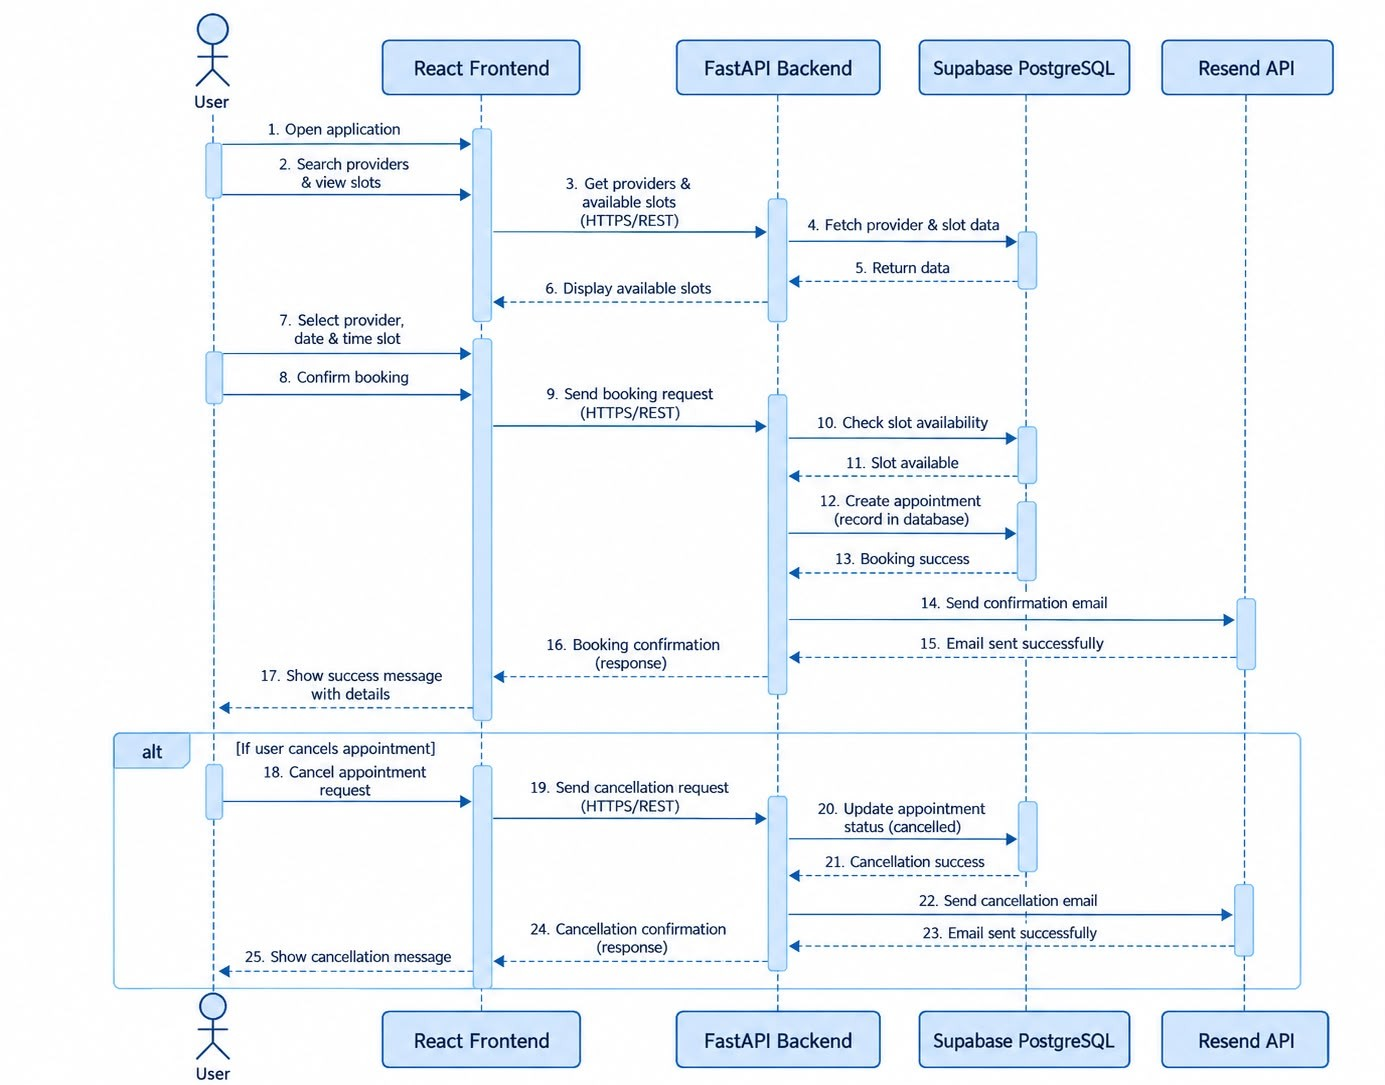
\includegraphics[width=0.88\textwidth]{4.2.jpeg}
\caption{Appointment Booking Sequence Diagram}
\label{fig:booking-sequence}
\end{figure}

% ------------------------------------------------------------
\section{Database Design}
\label{sec:database}

\subsection{Entity Relationships}
\label{subsec:er}

The database contains eight tables linked by foreign key relationships. The central entity is \texttt{public.users}, which extends Supabase's \texttt{auth.users} table. All other user data tables reference \texttt{users} with cascade deletion. The relationships are described in Table~\ref{tab:er}. Figure~\ref{fig:er} presents the entity-relationship diagram.

\begin{figure}[h!]
\centering
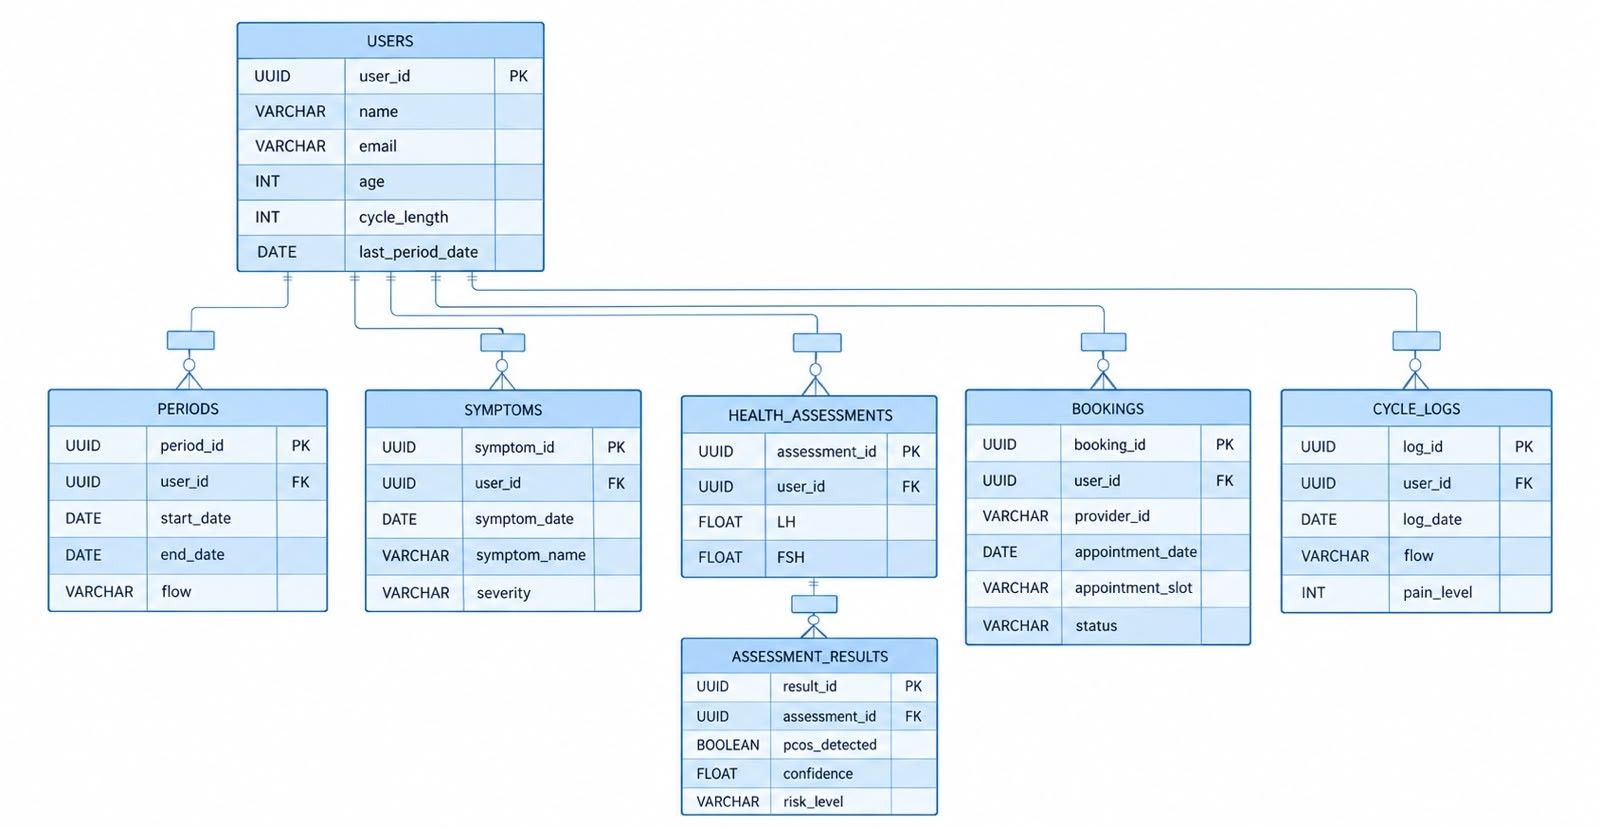
\includegraphics[width=0.88\textwidth]{4.3.jpeg}
\caption{Entity-Relationship Diagram of FEMCARE}
\label{fig:er}
\end{figure}

\begin{table}[h!]
\centering
\caption{Table Relationships}
\label{tab:er}
\renewcommand{\arraystretch}{1.4}
\begin{tabular}{|p{3.5cm}|p{2.5cm}|p{6.5cm}|}
\hline
\rowcolor[HTML]{D9D9D9}
\textbf{Table} & \textbf{Relationship} & \textbf{Notes} \\
\hline
auth.users $\rightarrow$ users & 1:1 & Trigger auto-creates profile on signup \\
\hline
users $\rightarrow$ cycle\_logs & 1:N & Unique per (user\_id, log\_date) \\
\hline
users $\rightarrow$ periods & 1:N & Unique per (user\_id, start\_date) \\
\hline
users $\rightarrow$ symptoms & 1:N & Keyed by (user\_id, symptom\_date) \\
\hline
periods $\rightarrow$ cycle\_history & 1:1 & Auto-populated by trigger \\
\hline
users $\rightarrow$ health\_assessments & 1:N & Stores raw ML input features \\
\hline
health\_assessments $\rightarrow$ assessment\_results & 1:1 & Stores ML prediction output; immutable \\
\hline
users $\rightarrow$ bookings & 1:N & Partial unique index on confirmed slots \\
\hline
\end{tabular}
\end{table}

\subsection{Key Table Design Decisions}
\label{subsec:table-design}

Several design decisions in the schema are worth noting at this level:

\begin{itemize}
    \item \textbf{cycle\_logs} stores \texttt{symptoms} and \texttt{moods} as PostgreSQL text arrays, reflecting the multi-select nature of the logging interface. The \texttt{symptoms} table stores the same data in a normalised, one-row-per-symptom form to support per-symptom queries on the Dashboard.

    \item \textbf{health\_assessments} column names match the feature names in the serialised XGBoost model file exactly. This ensures that the DataFrame constructed in the backend aligns with the model without any column remapping.

    \item \textbf{assessment\_results} has no UPDATE or DELETE RLS policy, making assessment history immutable by design.

    \item \textbf{cycle\_history} is populated automatically by a PostgreSQL trigger (\texttt{calculate\_cycle\_metrics}) that fires after an insert or update on \texttt{periods}, computing cycle length as the interval between consecutive period start dates.

    \item \textbf{bookings} uses a partial unique index rather than a table-level constraint so that the same slot can be re-booked after cancellation, since cancelled rows are excluded from the uniqueness check.
\end{itemize}

\subsection{Row Level Security}
\label{subsec:rls}

Every user data table has RLS enabled. All SELECT, INSERT, UPDATE, and DELETE policies are conditioned on \texttt{auth.uid() = user\_id}, ensuring that Supabase client queries from the frontend are automatically scoped to the authenticated user without relying on application-layer filtering. Assessment results have SELECT-only RLS; they cannot be modified or deleted through the client.

% ------------------------------------------------------------
\section{AI and ML Component Design}
\label{sec:ai-design}

\subsection{PCOS Assessment Pipeline}
\label{subsec:pcos-design}

The PCOS assessment is designed as a two-stage pipeline. In the first stage, the frontend collects 18 feature values through a guided wizard and derives the LH/FSH ratio automatically. In the second stage, the backend loads the serialised XGBoost pipeline (\texttt{cycle\_prediction\_xgboost\_pipeline.pkl}) and a feature-name list (\texttt{pcos\_features.pkl}) at application startup. At inference time, the input values are assembled into a pandas DataFrame, columns are aligned to the model's expected feature order using the loaded feature list, and the model's \texttt{predict} and \texttt{predict\_proba} methods produce the binary classification and confidence score. The risk level (Low, Moderate, or High Risk) is derived from the predicted class and confidence. A heuristic scoring function counts clinically relevant PCOS markers and serves as the fallback when the model cannot be loaded. Figure~\ref{fig:pcos-assessment} illustrates this assessment workflow.

\begin{figure}[h!]
\centering
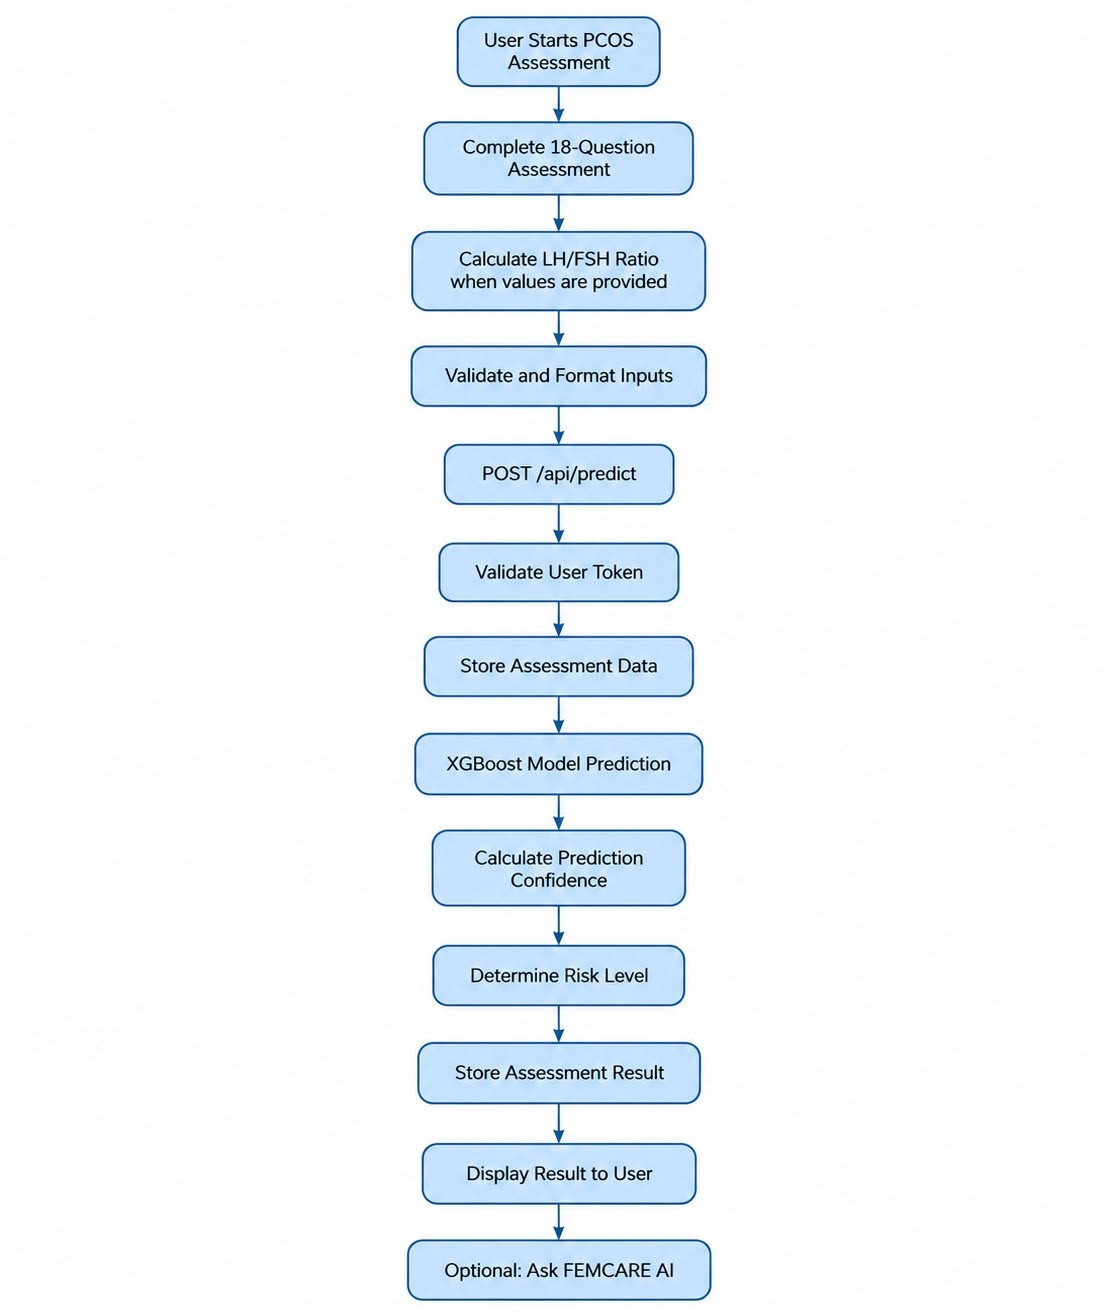
\includegraphics[width=0.25\textwidth]{4.4.jpeg}
\caption{PCOS Assessment Workflow}
\label{fig:pcos-assessment}
\end{figure}

\subsection{AI Health Assistant Pipeline}
\label{subsec:chat-design}

The chatbot is implemented as a sequential pipeline in \texttt{femcare\_chatbot.py}. The pipeline has five stages:

\begin{enumerate}
    \item \textbf{Scope check} -- A keyword-based filter tests the message against a set of out-of-scope categories (programming, sports, weather, entertainment). If any health-related keyword is also present, the message is considered in scope regardless of other matches.
    \item \textbf{Urgency check} -- If urgency keywords are detected (e.g. severe pain, fainting), an urgency instruction is appended to the system prompt.
    \item \textbf{Knowledge retrieval} -- A topic is detected from the message and the corresponding entry from the structured knowledge base is formatted as context.
    \item \textbf{User context enrichment} -- If the user is authenticated, their last period date and recent symptoms are fetched from Supabase and appended to the user turn.
    \item \textbf{LLM call} -- The Groq API is called with the FEMCARE system prompt and the assembled user content. Temperature is set to 0.4 and \texttt{max\_tokens} to 400 to produce concise, medically cautious responses. \cite{maity2025}
\end{enumerate}

% ------------------------------------------------------------
\section{Security Design}
\label{sec:security-design}

The security design of FEMCARE operates at three levels:

\textbf{Authentication.} User identity is managed by Supabase Authentication. The platform issues short-lived JWTs that are automatically refreshed by the client. Passwords are stored and verified exclusively within Supabase's authentication service and are never accessible to the application layer.

\textbf{Authorisation and data isolation.} As described in Section~\ref{subsec:rls}, RLS policies enforce per-user data access at the database level. The backend validates the Bearer token on every protected endpoint by calling \texttt{supabase.auth.get\_user(token)} before any database operation. This ensures that a user cannot access or modify another user's bookings, assessments, or health logs even if they possess a valid JWT.

\textbf{Credential management.} All service credentials -- the Supabase service role key, GROQ\_API\_KEY, and RESEND\_API\_KEY -- are stored in a server-side \texttt{.env} file and loaded at runtime via \texttt{python-dotenv}. \cite{kotz2016}

% ------------------------------------------------------------
